\documentclass[xcolor=dvipsnames]{beamer}

\usepackage{amsmath}
\usepackage{listings}
\usepackage{outlines}
\usepackage{graphicx}
\usepackage{amsfonts}
\usepackage{bbm}
\usepackage{ulem}

\usetheme{Madrid}
\useoutertheme{miniframes} % Alternatively: miniframes, infolines, split
\useinnertheme{circles}

\definecolor{IITHorange}{RGB}{243, 130, 33} % UBC Blue (primary)
\definecolor{IITHyellow}{RGB}{254, 203, 10} % UBC Grey (secondary)

\setbeamercolor{palette primary}{bg=IITHorange,fg=white}
\setbeamercolor{palette secondary}{bg=IITHorange,fg=white}
\setbeamercolor{palette tertiary}{bg=IITHorange,fg=white}
\setbeamercolor{palette quaternary}{bg=IITHorange,fg=white}
\setbeamercolor{structure}{fg=IITHorange} % itemize, enumerate, etc
\setbeamercolor{section in toc}{fg=IITHorange} % TOC sections

% Override palette coloring with secondary
\setbeamercolor{subsection in head/foot}{bg=IITHyellow,fg=white}

\definecolor{codegreen}{rgb}{0,0.6,0}
\definecolor{codegray}{rgb}{0.5,0.5,0.5}
\definecolor{codepurple}{rgb}{0.58,0,0.82}
\definecolor{backcolour}{rgb}{0.95,0.95,0.92}

\lstdefinestyle{mystyle}{
    backgroundcolor=\color{backcolour},   
    commentstyle=\color{codegreen},
    keywordstyle=\color{magenta},
    numberstyle=\tiny\color{codegray},
    stringstyle=\color{codepurple},
    basicstyle=\ttfamily\footnotesize,
    breakatwhitespace=false,         
    breaklines=true,                 
    captionpos=b,                    
    keepspaces=true,                 
    numbers=left,                    
    numbersep=5pt,                  
    showspaces=false,                
    showstringspaces=false,
    showtabs=false,   
    tabsize=2
}
\lstset{style=mystyle}

\title[Report 20/05]{Report 20/05}

\begin{document}
	
	\begin{frame}
		\titlepage
	\end{frame}
	

	\section{Introduction}

	\begin{frame}{Introduction}
        This presentation shows a summary of the work done in the past few weeks. It includes the models used and the results obtained.
        

        \textit{This document is for internal use, so it may contain some errors.}

	\end{frame}

    \section{Validation}



    \subsection{Validate the models on the period (2020-2023)}

    \begin{frame}
        \begin{figure}
            \centering
                 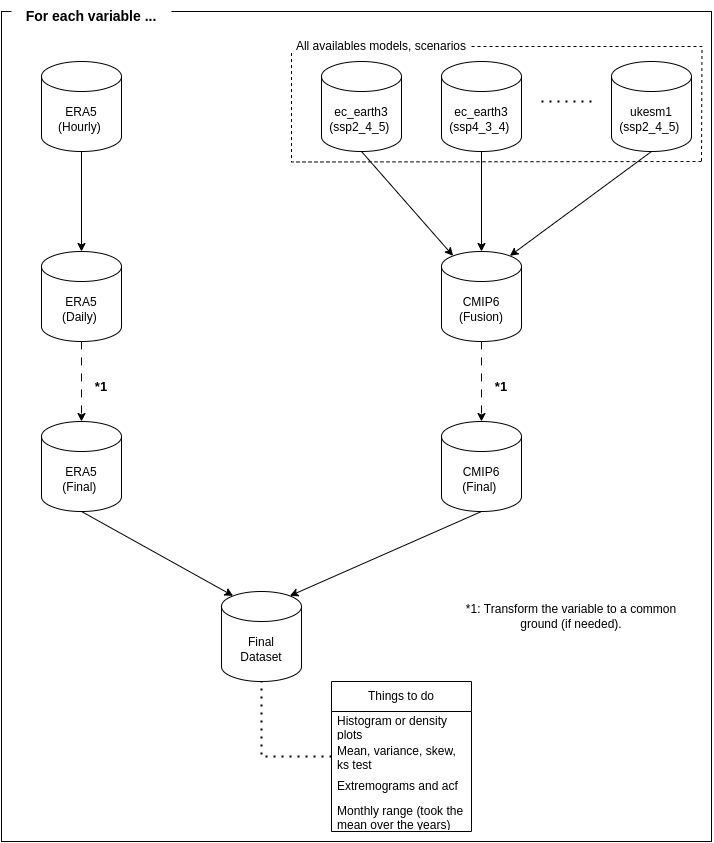
\includegraphics[width=0.57\textwidth]{images/diagram.png}
            \label{fig:series}
        \end{figure}
    \end{frame}

    \section{Downscaling: Train Models}

    \begin{frame}
        \begin{outline}
            \1 We train the models with the era5 data only. Split the data in train/validation/test. (2000-2013) train, 2014 test.            
            \1  If we choose to use all the variables as a predictor, we need to look for the variables that are available in both models. Also we need to check if are measured in the same way or a transformation is needed. Also we need to define the period, right now we are only working with the data between 2000-2014, but we can expand this period.
            \1 With the predicted result for the test, we can measure the errors of the model using our metrics. (We need to define if in this step we use paired or non paired metrics). 
            \1 Right now the models are naive, xgboost, lstm and cnn (knn was discarded (?)). LSTM and CNN gave good results so we are going to focus on NN models.
           \end{outline}
    \end{frame}

    \section{Downscaling: Apply Models}

    \begin{frame}
        \begin{outline}
            \1 We apply the models trained with the era5 data to the cmip data.
            \1 We need to define if we are gonna preserve the cmip values or we are gonna use the predicted values without considering the conservation of the aggregated values.
            \1 With the downscaled data we can use our metrics (non paired) to evaluate the performance (taking into account the work done at the validation part).
        \end{outline}
    \end{frame}

    \section{Things to do}
    \begin{frame}
        \begin{outline}
            \1 Validation
            \1 Look for the predictors that are available in both models.
            \1 Look for new NN models (\sout{Convolutional NN}, ...).
            \1 Preservation vs Non preservation
        \end{outline}
    \end{frame}
    
\end{document}
